\documentclass[a4paper, english]{article}

% includes 
% Language setting
\usepackage[english]{babel}
\usepackage{csquotes}
\usepackage[iso]{isodate}
\usepackage[version=4]{mhchem} % for chemical reaction formulas
% Set page size and margins
\usepackage[a4paper,top=2cm,bottom=2cm,left=3cm,right=3cm,marginparwidth=1.75cm]{geometry}
%% images
\usepackage{graphicx}
\usepackage{wrapfig}
%% captions 
\usepackage{caption}
\usepackage{subcaption}
%% tables 
\usepackage{booktabs}
%% colors
\usepackage{xcolor}
%% links and refs and citations 
\usepackage[colorlinks=true, allcolors=blue]{hyperref}
\usepackage[capitalize]{cleveref}
\usepackage[backend=biber]{biblatex}
%% acronyms and glossary 
\usepackage[automake,acronyms,xindy,translate=babel]{glossaries} % TODO 
\usepackage{glossaries-extra}
%\usepackage{acro}
%% include code snippets
\usepackage{listings}
%% maths
\usepackage{amsmath}
%% title page
\usepackage{titling} % for cooler titlepages 

% configuration 
\bibliography{refs.bib} % Entries are in the refs.bib file
% configure python code snippets
\lstdefinestyle{PyStyle}{%
    commentstyle=\color{olive},
    keywordstyle=\color{magenta},
    numberstyle=\tiny\color{gray},
    stringstyle=\color{purple},
    basicstyle=\footnotesize,
    breakatwhitespace=false,         
    breaklines=true,                 
    captionpos=b,                    
    keepspaces=true,                 
    numbers=left,                    
    numbersep=5pt,                  
    showspaces=false,                
    showstringspaces=false,
    showtabs=false,                  
    tabsize=2,
    language=python
}
% setup title 
\title{\textit{} \\ \vspace{1cm}Project Report \\ \vspace{1cm} \textbf{\huge Impact of Climate and Land Cover Change in Urban Heat Islands}\\ \vspace{1.2cm} }
\author{Linus Andrae (6015384)}
\date{\today}

\makeglossaries%
% Acros
\newabbreviation{USGS} {USGS} {United States Geological Survey}
\newabbreviation{LST}  {LST}  {Land Surface Temperature}
\newabbreviation{LULC} {LULC} {Land Use/ Land Cover}
\newabbreviation{UHI}  {UHI}  {Urban Heat Island}
\newabbreviation{NDVI} {NDVI} {Normalized Differential Vegetation Index}
\newabbreviation{NIR}  {NIR}  {Near Infrared}
\newabbreviation{OSM}  {OSM}  {Open Street Map}
\newabbreviation{TOA}  {TOA}  {Top of Atmosphere}
\newabbreviation{ECMWF}{ECMWF}{European Center for Medium-Range Weather Forcasts}

\begin{document}
  \begin{titlingpage} %This starts the title page
\pagenumbering{Alph}
\thispagestyle{empty} 
\begin{center}
\begin{large}
  \textit{University Bremen}\\
\end{large}
\vspace{4cm} %You can control the vertical distance
\begin{large} 
\textbf{\thetitle} 
\end{large}
\theauthor\\
\thedate\\
\vspace{13cm} %Put the distance you need.


\includegraphics[width=0.3\textwidth]{img/res/uniLogoIUP.png}
\hspace{4cm}

\includegraphics[width=0.3\textwidth]{img/res/logo_ohb_digital.png}

\end{center}
\end{titlingpage}
\pagenumbering{arabic}

  \newpage

  \begin{abstract}
\noindent
Urban Heat Islands (\acp{UHI}) pose a growing health risk by exacerbating heat stress for residents of urban areas. 
Due to the increased prevalence of extreme weather events and heat waves and as a cause for higher energy consumption, \acp{UHI} become more relevant as a topic for city planners and policy makers to consider.
Identification of areas most impacted or at risk require a data backed tool set to aid urban planning. 
This study presents a comprehensive pipeline developed using Python to automate the processing and analysis of Landsat 7,8 and 9 remote sensing imagery.
The pipeline facilitates the generation of Normalized Difference Vegetation Index (NDVI) and heat maps, running statistical analysis of factors known to create \acp{UHI} of a provided area of interest, serving as a robust toolset for the investigation and detection of \acp{UHI}.
The methodology employed leverages the spectral characteristics of Landsat data to provide high-resolution insights into temperature variations within urban areas as well as statistical analysis of the composition of the identified Urban Heat Islands.
The ultimate aim is to offer actionable guidance to city planners and developers for the mitigation of \acp{UHI}, by classification of \acp{UHI} on different scales.
At the current implementation level the pipeline is able to detect \acp{UHI} from level one brightness temperature and the statistical analysis indicate a strong correlation between land cover types and heat island intensity, affirming the utility of the pipeline in urban climate studies.
%To analyse and identify Urban Heat Islands using remote sensing imagery
\end{abstract}

  \newpage
  % TODO insert Eigenständigkeitserklärung

  \tableofcontents
  \listoffigures
  \listoftables

  \section*{Acronyms}
  \printglossaries%
  %\begin{acronym}
      %\end{acronym}
\newpage

\section{Introduction}
    \subsection{Background}
   \section{Background}
\subsection{Urban Heat Islands}
The phenomenon of \acp{UHI} has been studied for the past 30 years. 
Due to increase in global temperature as well as increased occurrence of extreme weather and periods of heatwaves, this phenomenon will likely increase in intensity and will also occur in cities at higher latitudes~\cite{Sachindra2016}\cite[p.~904]{Wilby2008}.
\acp{UHI} are a spacial phenomenon that occurs on different scales and intensities, this makes observation using remote sensing data a good and widely used approach~\cite{Weng2003}.\\
\acp{UHI} are distinguished into surface and atmospheric \acp{UHI}.
Within this context we will only investigate surface \acp{UHI}. 
Surface \acp{UHI} are areas of higher surface temperatures within urban areas compared to rural areas due to the materials used and heat from mobility, electrical appliances, heating and cooling as well as less vegetation and higher sealed surfaces that reduce surface water availability\cite[pp. 7-12]{EPA2008}. 
The surface \acp{UHI} are longer term phenomenon that are most intense in summer. 
Atmospheric \acp{UHI} are more dependent on weather and local topology and are in part a side effect of the slower cooling of the city air due to the higher thermal capacity and wind obstruction.
This phenomenon is not investigated by this work, since the air temperature can not be directly observed by remote sensing data.
%Under certain conditions the increased temperature will form a hot air pocket, that will trap the head and reduce airflow from and to the area. \\
The main factors in forming urban heat islands is the thermal storage capacity of materials used in urban areas like concrete, asphalt and steel, that have a high heat capacity and heat up quickly during the day and emit the stored thermal energy as sensible heat with a delay (eg.~during the night)\cite{Ramamurthy2014}. 
High surface sealing and lack of vegetation reduce surface water availability and diminish evaporation and the cooling effect of latent heat causing more thermal energy to be available as sensible heat. %todo source (sailor?  or first source)
Another factor is the heat produced by human activity such as industrial processes and combustion engines.
As a consequence of higher temperatures, active cooling devices are more frequently used for buildings and vehicles. 
The emitted thermal energy of these heat pumps further increases the surrounding temperature, reinforcing the effect.
\\
There are multiple adverse effects and possible mitigation techniques for the mitigation and reduction of urban heat islands have been studied extensively since the 1970s\cite{Nichol1994}\cite{Stewart2011}. % list studies.  
Advective cooling can be observed when the temperature gradient generated airflow from the cooler surrounding areas towards the hot areas within the city, cooling it down\cite{HaegerEugensson1999}. \\
Urban areas with no close water body (generating sea breezes as well as latent heat transport) and with lower average wind speed are more likely to be affected by urban heat islands\cite{Ramamurthy2017}. 
Higher temperatures due to \acp{UHI} cause stress to animals and humans increasing health risk due to heat stroke and increased surface level ozone concentration\cite{Santamouris2020}.
\subsection{Land Surface Temperature}
Land surface temperature is the temperature at which an object emits infrared radiation according to plank's law\cite{Liang2020}. 
Using remote sensing methods this quantity can not be directly observed since the satellite is observing \ac{TOA} brightness temperature. 
This temperature can be transformed to a \ac{LST} using atmospheric correction and correction for the emissivity of the ground.
The conversion factor is data source dependent and can be found in \cref{sec:lstcalc}.

    \subsection{Research Question}
    
    \subsection{Methodology}
    \subsection{Structure of the Thesis}

\section*{Acknowledgements}

\section{Theoretical Framework}
    \subsection{Definitions}
    \subsection{Indices}
Many different indices are used for analysis of images or parameters in remote sensing, atmospheric physics and meteorology.
The following sections introduce the indices that where used to analyse the \glspl{UHI} within this work. 
\subsubsection{NDVI}
\textit{The following section is a slightly reworked version of a section from the pre-thesis master project~\cite{andrae2023}}\\ 
%
\noindent
\begin{figure}[!htbp]
    \centering
    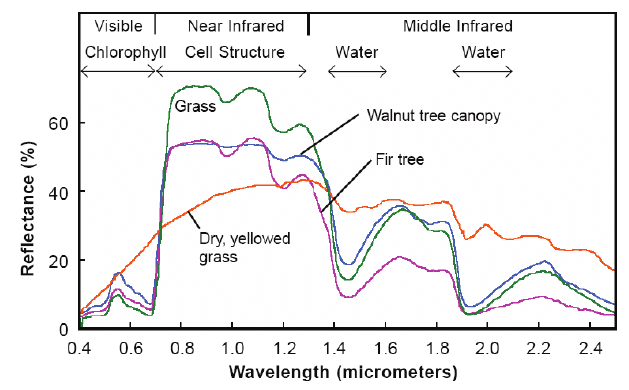
\includegraphics[width=0.5\textwidth]{img/Reflectance-spectra-of-different-types-of-green-vegetation-compared-to-a-spectral.png}
    \caption{Absorption spectrum of green vegetation \autocite[P. 5]{Smith2012}\label{fig:absorbtionVeg}}
\end{figure}
The \gls{NDVI} is an widely used index using the difference of the red and near infrared bands to determine the amount of green vegetation. 
\begin{equation}
    NDVI = \frac{Red-NIR}{Red+NIR}
    \label{equ:ndvi}
\end{equation}
For Landsat 8 and 9 data, channel 4 (red $640\ \text{nm} - 670\ \text{nm}$) and channel 5 (near infrared $850\ \text{nm} - 880\ \text{nm}$) where used.
As shown in \cref{fig:absorbtionVeg} healthy plants reflect near infrared and there is a sharp rise in reflectance between the two used channels at around $700\ \text{nm}$. 
%
This index is used for emissivity estimation for Land Surface Temperature calculation see \cref{equ:toa}, correlation with heat islands (since there is a negative correlation between those two values, due to the latent heat of evaporation reducing surface temperature at higher vegetation areas).
\begin{figure}[!htbp]
    \centering
    \begin{subfigure}{0.45\textwidth}
    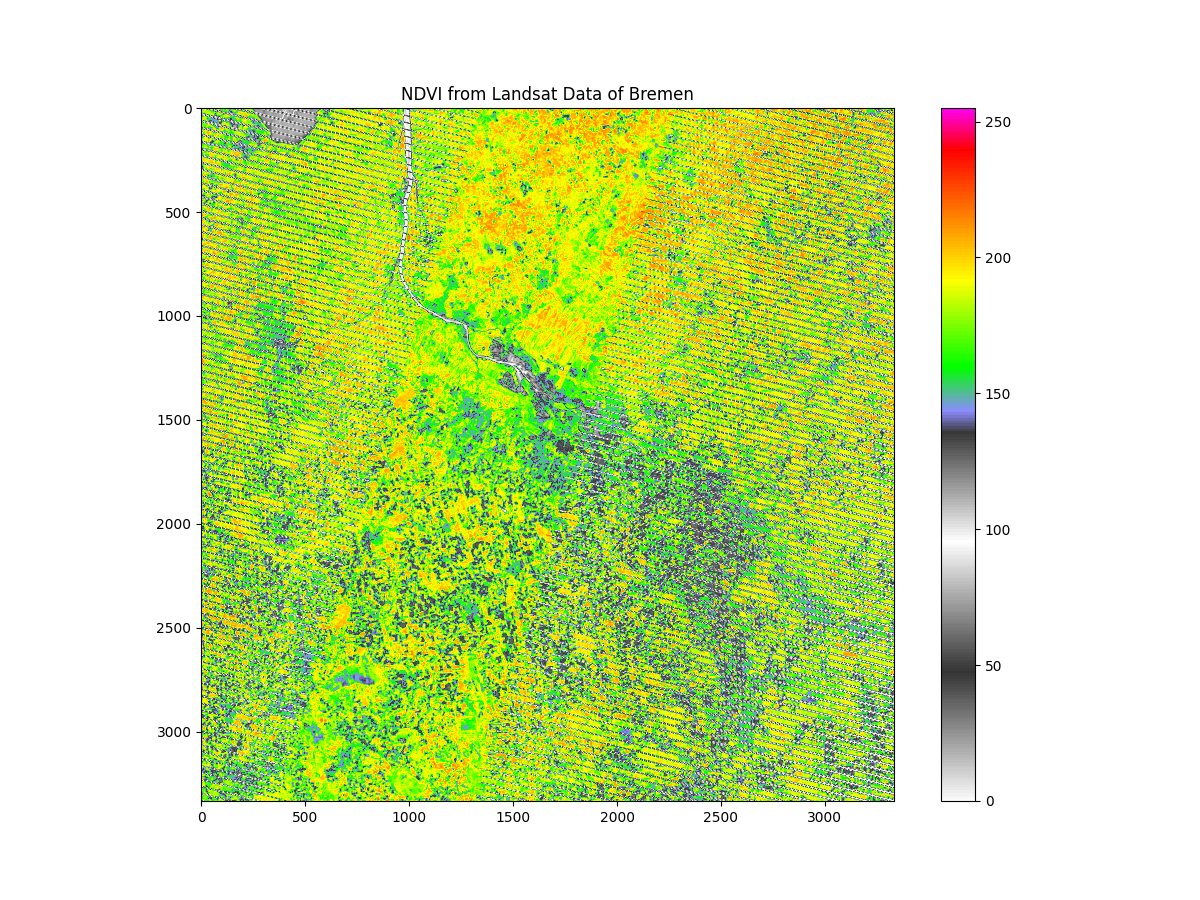
\includegraphics[width=\textwidth]{img/NDVI_LE07_L1TP_196023_20190723_20200825_02_T1__Bremen.png}
    \subcaption{NDVI of Bremen (Bands 5 and 6) using Landsat 7 data on 2019--07--23}
    \end{subfigure}
    \begin{subfigure}{0.45\textwidth}
    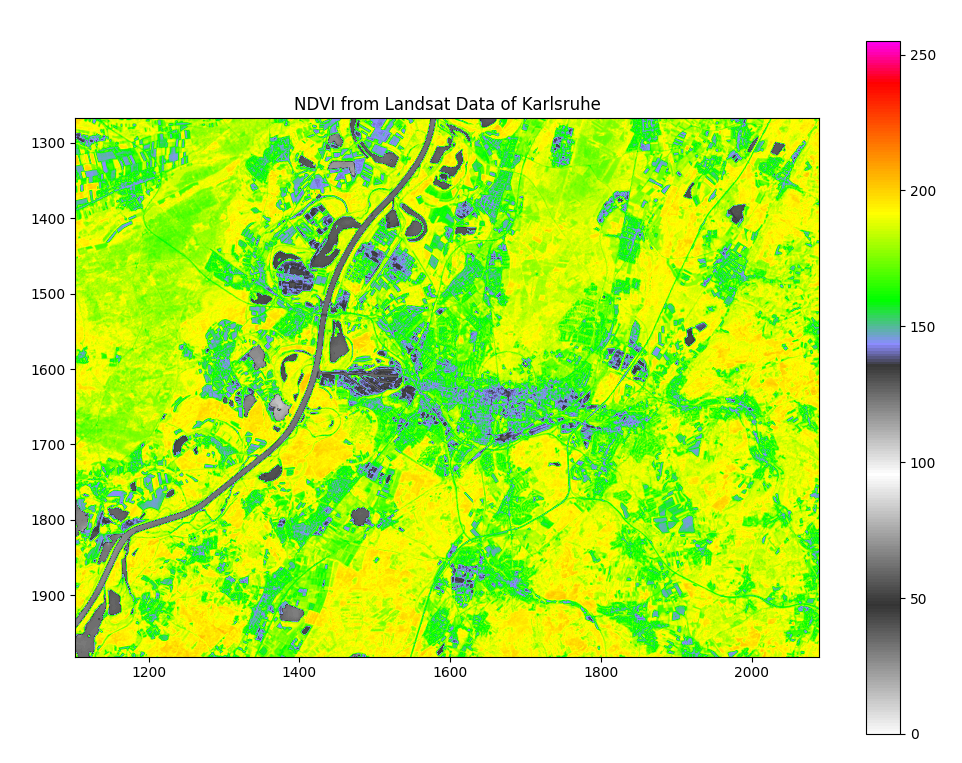
\includegraphics[width=\textwidth]{img/KarlsruheNDVI_Landsat8.png} 
    \subcaption{NDVI of Karlruhe (Bands 4 and 5) using Landsat 8 data on 2023--06--07}
    \end{subfigure}
    \caption{NDVI Images from the different satellites\label{fig:ndvi}}
\end{figure}
%\subsubsection{NDVI Colormap}\label{sec:colormap}
%When using a classical heat map with a color gradient from colder to warmer colors or a diverging color map (see \cref{fig:ndviPhoenixAzBad}), details of the image get lost and it is hard to distinguish plant heath, build up and vegetated areas and the difference between small \gls{NDVI} changes.
%To aid an intuitive understanding a specially created colormap can be used. 
%The color map was adapted for use in python from work of \texttt{public lab}\cite{ndviCmap} where it was developed in an attempt to create color-blind friendly \gls{NDVI} color maps.
%Values below 0.2 are areas with no vegetation.
%The color map used in \cref{fig:ndviPhoenixAz} uses a gradient of gray with a ``black-white-black
%white'' transition to allow higher dynamic range for non vegetation areas.
%For areas with an \gls{NDVI} $<$ 0.2 blue is used. Green values are low or unhealthy green vegetation or mixed use pixels. 
%Orange and red values correspond to thicker vegetation e.g.~forests, parks or green fields. 
%%
%Comparing \cref{fig:ndviPhoenixAz}  and \cref{fig:ndviPhoenixAzBad} where most of the desert surrounding the city has no green vegetation and the parts covered in vegetation can be clearly distinguished from the arid desert regions.
%Still the surface roughness can be seen quite well due to the gray scale gradient in the $<$ 0.2 \gls{NDVI} range.  
%%
%\begin{figure}[htbp]
% \centering
%    \begin{subfigure}{0.46\textwidth}
%    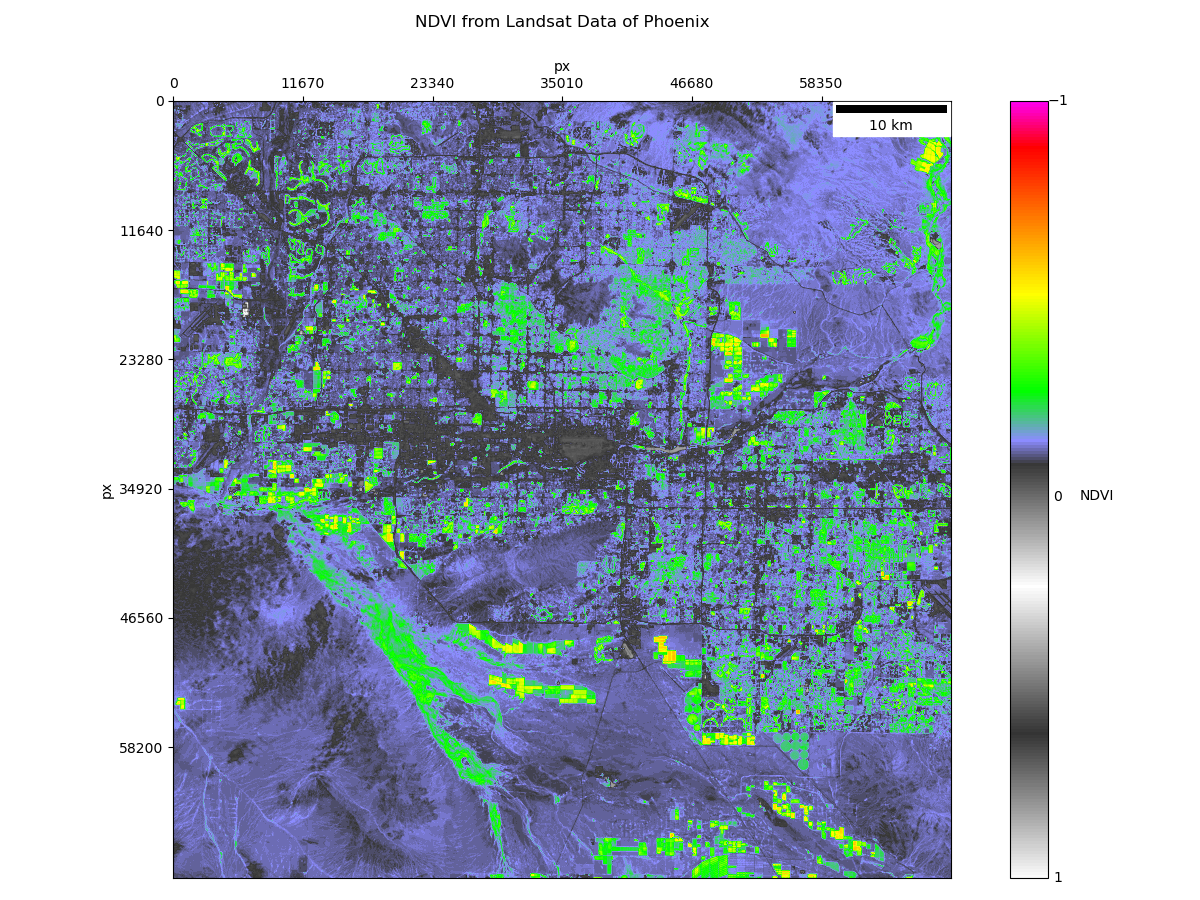
\includegraphics[width=\textwidth]{img/NDVI from Landsat Data of Phoenix.png} 
%    \subcaption{NDVI Image of Phoenix with the  VGYRM color map\label{fig:ndviPhoenixAz}}
%    \end{subfigure}
%    \begin{subfigure}{0.46\textwidth}
%    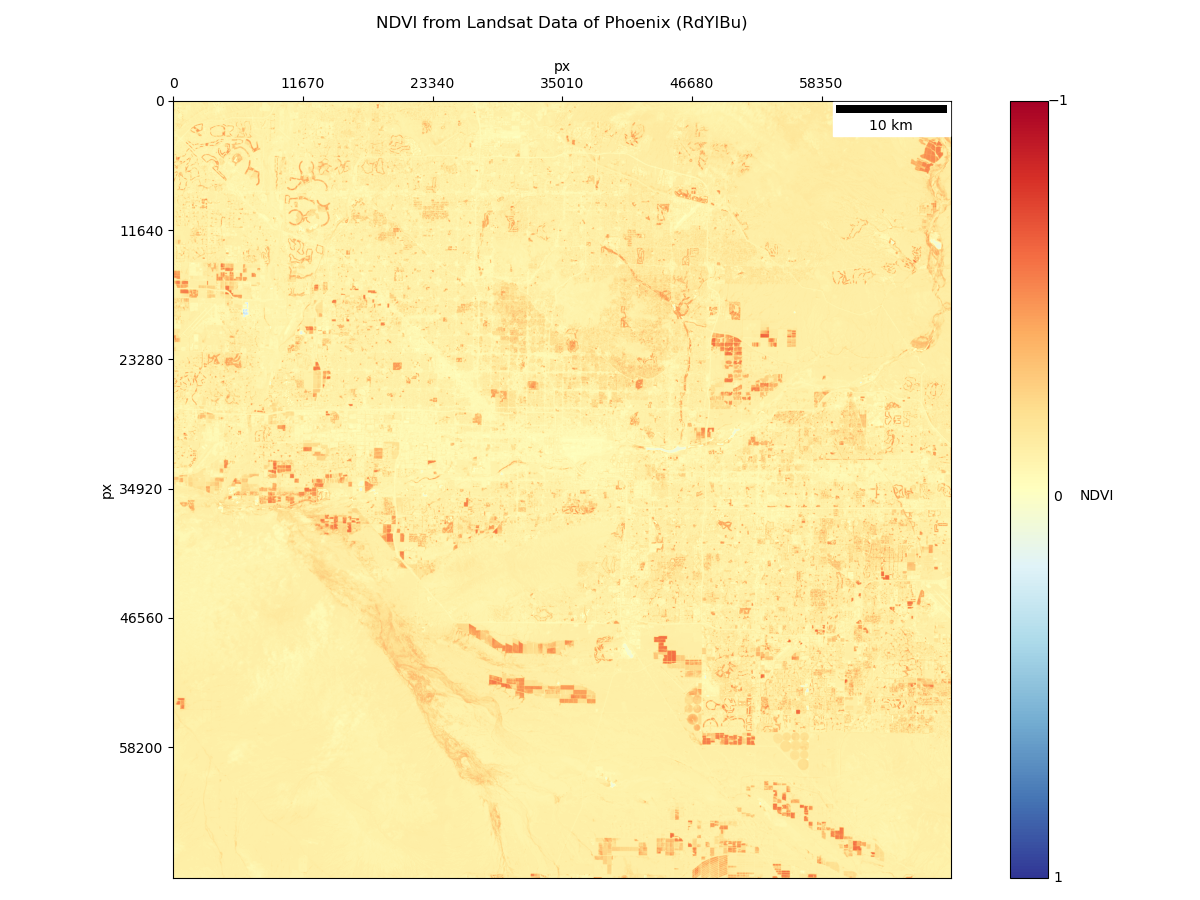
\includegraphics[width=\textwidth]{img/NDVI from Landsat Data of Phoenix (RdYlBu).png} 
%    \subcaption{NDVI Image of Phoenix with a RdYlBu gradient color map\label{fig:ndviPhoenixAzBad}}
%    \end{subfigure}
%    \caption{Different color maps used show the better ability to differentiate between green vegetation and desert and buildings within Phoenix\label{fig:ndvicomp}}
%\end{figure}

    \subsubsection{Wet Bulb Globe Temperature}
    The human body reacts to heat stress differently in different environmental conditions. 
    Working under heat stress poses a serious health issue, for this the \gls{WBGT} was defined as EN ISO 7243:2017, calculating the thermal load on the human body\cite{isoWBGT}
    Heat exchange between the human body and the environment is dominated by evaporation of secreted sweat.
    The efficiency of this process is determined by the vaporation pressure, that is influenced by temperature difference and the humidity difference. %TODO ref paper with caves
    The Heat Index is a simple way of calculating this efficiency that does not take radiant heat into account, the WBGT does incorperate this effect as well as clothing in this process. 


    
    \subsection{Models and Theories}


\section{Comparable Definition of Urban Heat Islands}
    \subsection{Introduction}
    The definitions of \glspl{UHI} in the literature are varying slightly and do not take into account that, using remote sensing techniques most definitions do not allow easy comparison between different areas or times.
    %TODO add sources, maybe add examples? 
    The definition of the U.S.~EPA\cite{epaUHIDef} and the German Weather Service (DWD) both say it is an feature defined by increased temperature between the urbanized areas compared to the sourrounding. % TODO cite  
    Different studies analyzing \glspl{UHI} use difference referenece tempereatures.
    The first goal of this work is defining a systematic reproducable aproach to measure urban heat island intensity based on land usage. 
    \subsection{Approach}
    To make the approach comparable previous work was done takeling the problem using a comparable definition for comparing \gls{SUHI} around the world using Sentinel images\cite{Sobrino2020}.
    The landcover indicating urban areas is identified and the urban area polygon is extended by buffer zones. 
    In~\cite{Sobrino2020} urban adjacent, future urban adjacent and peri-urban areas are defined.
    The used approach was adapted by removing the urban growth projection (the paper investigated \glspl{SUHI} in 2050).
    For \gls{LULC} Landsat 8/9 data was used combined with a SVM (see \cref{sec:svm}). 

    

    \subsection{Analysis}
    \subsubsection{SVM}\label{sec:svm}
    For classifing surfaces a \gls{SVM} was used, that utilized multiple multispectral input images of the same city at different seasons as training material.
    The SVM uses a lagrange multiplication to optimize a minimiziation problem for a grouping a given set of multi-dimentional parameters. 
    In the case of the used multi spectral landsat dataset, the value of each image pixel for each band is used creating a vector of band 1--7 of the OLI instrument. 
    
    
    \subsection{Conclusions}

\section{Impact of Climate Change on UHIs}
    \subsection{Introduction}
    \subsection{Analysis}
    \subsection{Conclusions}

\section{Impact of Land Use Land Cover Changes on UHIs}
    \subsection{Introduction}
    \subsection{Analysis}
    \subsection{Conclusions}

\section{Simulation and Modeling of UHIs}
    \subsection{Introduction}
    \subsection{Analysis}
    \subsection{Conclusions}

\section{Discussion}
    \subsection{Synthesis of Findings}
    \subsection{Implications}

\section{Conclusion}
    \subsection{Summary}
    \subsection{Future Work}

\section{Appendix}
    \subsection{Data}
    \subsection{Code}


\newpage
\printbibliography
\end{document}

%The surface classes where correlated with the %TODO check 
%Kataster data from Bremen as well as with OSM data. % todo do 
%
%Ziel Projekt teil: 
%- detection and error margins in UHI detection using remote sensing data 
%- data pipeline to create maps of UHI in areas 
%- surface classification based on remote sensing data correlated with 2nd and 3rd sources (kataster/ OSM) 
%- UHI "cores" identification 
%
%Master Fragestellungen: 
%- Correlation zw. UHI} und Pollutants? 
%https://pubs.acs.org/doi/epdf/10.1021/cr5006815 
%- Real time UHI size/occurrence prediction based on ground temperature stations (Bremen Airport) and pollutant levels? 
%- UHI classification in different environments, causes and effects, mitigation stategies? (e.g. Classification of Surface types, vegetation etc. within different climate zones (Phoenix, Bremen, Karlruhe, Essen, Something meditareiean, Afrika (coastal, arid, etc) /paper with adis abbeba)
%
%\subsection{}

%Of the different bands available from the used satellite data (Landsat7 and Landsat8), 
%the visible and near infrared bands where used for clustering. 
%The clustering was done using the simple k-means algorithm. 
%Different configuration where used %todo add pictures? 
%These where compared and referenced with ground truth data %todo add error and limitations refgerenec here 


